\documentclass[miniframe]{lbpbeamer}
%\documentclass[handout]{lbpbeamer}
%%%%%%%%%%%%% option de la classe lbpbeamer.cls
% toutes les options standards de la classe beamer
% le type d'en-tete pour l'appel des sections : 
%  - default : currentsection | currentsubsection
%  - miniframe : sections + puces
%  - tree : sections + currentsubsection
%  - split : sections + subsections
%%%%%%%%%%%%%%%%%%%%%%%%%%%%%%%%%%%%%%%%%%%%%%%%%%

%%%%%%%%%%%%% appel des packages
\usepackage[english,french]{babel}
\usepackage{epsfig}
\usepackage[T1]{fontenc}
\usepackage[utf8]{inputenc}
\usepackage{lmodern} 
\usepackage{times}
\usepackage{multirow}
\usepackage{animate}
\usepackage{hyperref}
\usepackage{movie15}
\usepackage{wasysym}
\usepackage[squaren, Gray, cdot]{SIunits}
\usepackage{tikz}
\usetikzlibrary{calc,trees,positioning,arrows,chains,shapes.geometric,%
	decorations.pathreplacing,decorations.pathmorphing,shapes,%
matrix,shapes.symbols,plotmarks,decorations.markings,shadows}

\usepackage{tabularx}
\newcolumntype{L}[1]{>{\raggedright\let\newline\\\arraybackslash\hspace{0pt}}m{#1}}
\newcolumntype{C}[1]{>{\centering\let\newline\\\arraybackslash\hspace{0pt}}m{#1}}
\newcolumntype{R}[1]{>{\raggedleft\let\newline\\\arraybackslash\hspace{0pt}}m{#1}}

\newcommand{\backupbegin}{
	\newcounter{framenumberappendix}
	\setcounter{framenumberappendix}{\value{framenumber}}
}
\newcommand{\backupend}{
	\addtocounter{framenumberappendix}{-\value{framenumber}}
	\addtocounter{framenumber}{\value{framenumberappendix}} 
}

%\usepackage{enumitem}

%%%%%%%%%%%%%%%%%%%%%%%%%%%%%%%%%%%%%%%%%%%%%%%%%%
%\newlist{fleche}{itemize}{1}
%\setlist[fleche]{label=$\rightarrow$,font=\color{blue}}


%\newcommand{\smiley}{\tikz[baseline=-0.75ex,black]{
%		    \draw circle (2mm);
%			\node[fill,circle,inner sep=0.5pt] (left eye) at (135:0.8mm) {};
%			\node[fill,circle,inner sep=0.5pt] (right eye) at (45:0.8mm) {};
%			\draw (-145:0.9mm) arc (-120:-60:1.5mm);
%			    }
%			}

\newcommand{\orto}{^{\circ}}

%%%%%%%%%%%%% appel du plan a chaque subsection
%% en 1 colonne

\AtBeginSection[]{
	\frame{%<handout:0>{
	\frametitle{Plan}
  \begin{columns}[t]
  \begin{column}{0.5\linewidth}
  \tableofcontents[sections={1-3}, currentsection,subsectionstyle=show/show/shaded]
  \end{column}
  \begin{column}{0.5\linewidth}
  \tableofcontents[sections={4-6}, currentsection,subsectionstyle=show/show/shaded]
  \end{column}
  \end{columns}
  }
}

%% ou en 2 colonnes s'il y a trop de sections
    
%\AtBeginSubsection[]{
%	\frame{%<handout:0>{
%	\frametitle{Summary}
%  \begin{columns}[t]
%  \begin{column}{0.5\linewidth}
%  \tableofcontents[sections={1-6},currentsection, subsectionstyle=show/shaded/hide]
%  \end{column}
%  \begin{column}{0.5\linewidth}
%  \tableofcontents[sections={7-12},currentsection,subsectionstyle=show/shaded/hide]
%  \end{column}
%  \end{columns}
%  }
%}	
%%%%%%%%%%%%%%%%%%%%%%%%%%%%%%%%%%%%%%%%%%%%%%%%%%	

%%%%%%%%%%%%% Pour supprimer les symboles de navigation
\setbeamertemplate{navigation symbols}{}
%%%%%%%%%%%%%%%%%%%%%%%%%%%%%%%%%%%%%%%%%%%%%%%%%%

%%%%%%%%%%%%% Personnalisation des theoremes
\newtheorem{theoreme}{Th\'eor\`eme}
\newtheorem{preuve}{D\'emonstration}
\newtheorem{define}{D\'efinition}
%%%%%%%%%%%%%%%%%%%%%%%%%%%%%%%%%%%%%%%%%%%%%%%%%%	
		
%%%%%%%%%%%%% Infos personnelles au document	
\title[Introduction à SysML]{Introduction à SysML}
\subtitle{Langage de modélisation graphique de systèmes}
\author[Fiack]{Laurent Fiack}
%\email{}
\institute[Lycée Blaise Pascal]{Lycée Blaise Pascal}
\date[\today]{\today}
\logo{}
%%%%%%%%%%%%%%%%%%%%%%%%%%%%%%%%%%%%%%%%%%%%%%%%%%

\newcommand{\figpath}{figures/}

\usepackage{scrextend}

\begin{document}

%%%%%%%%%%%%% Background des slides	
\usebackgroundtemplate{}
%% cet option permet d'ins\'erer une image en fond-ecran
%% la commande \usebackgroundtemplate{} permet de
%% supprimer le fond a partir du moment ou il est 
%% appele
%%%%%%%%%%%%%%%%%%%%%%%%%%%%%%%%%%%%%%%%%%%%%%%%%%	

%%%%%%%%%%%%% frame title
\frame{\titlepage}
\usebackgroundtemplate{}
\logo{}
%\logoheader{taille}{emplacement-image}
%% on supprime les logos des autres frames		
%%%%%%%%%%%%%%%%%%%%%%%%%%%%%%%%%%%%%%%%%%%%%%%%%%
\section[Chronologie]{Chronologie}
\frame{
	\frametitle{Premier jeu vidéo de l'histoire ?}
	\pause
	\begin{itemize}
		\item \textbf{1947:} Cathode-ray tube amusement device
			\begin{itemize}
				\item Simulateur de tir de missile
				\item Pas sorti des labos
			\end{itemize}
	\end{itemize}
	\pause
	\centering
	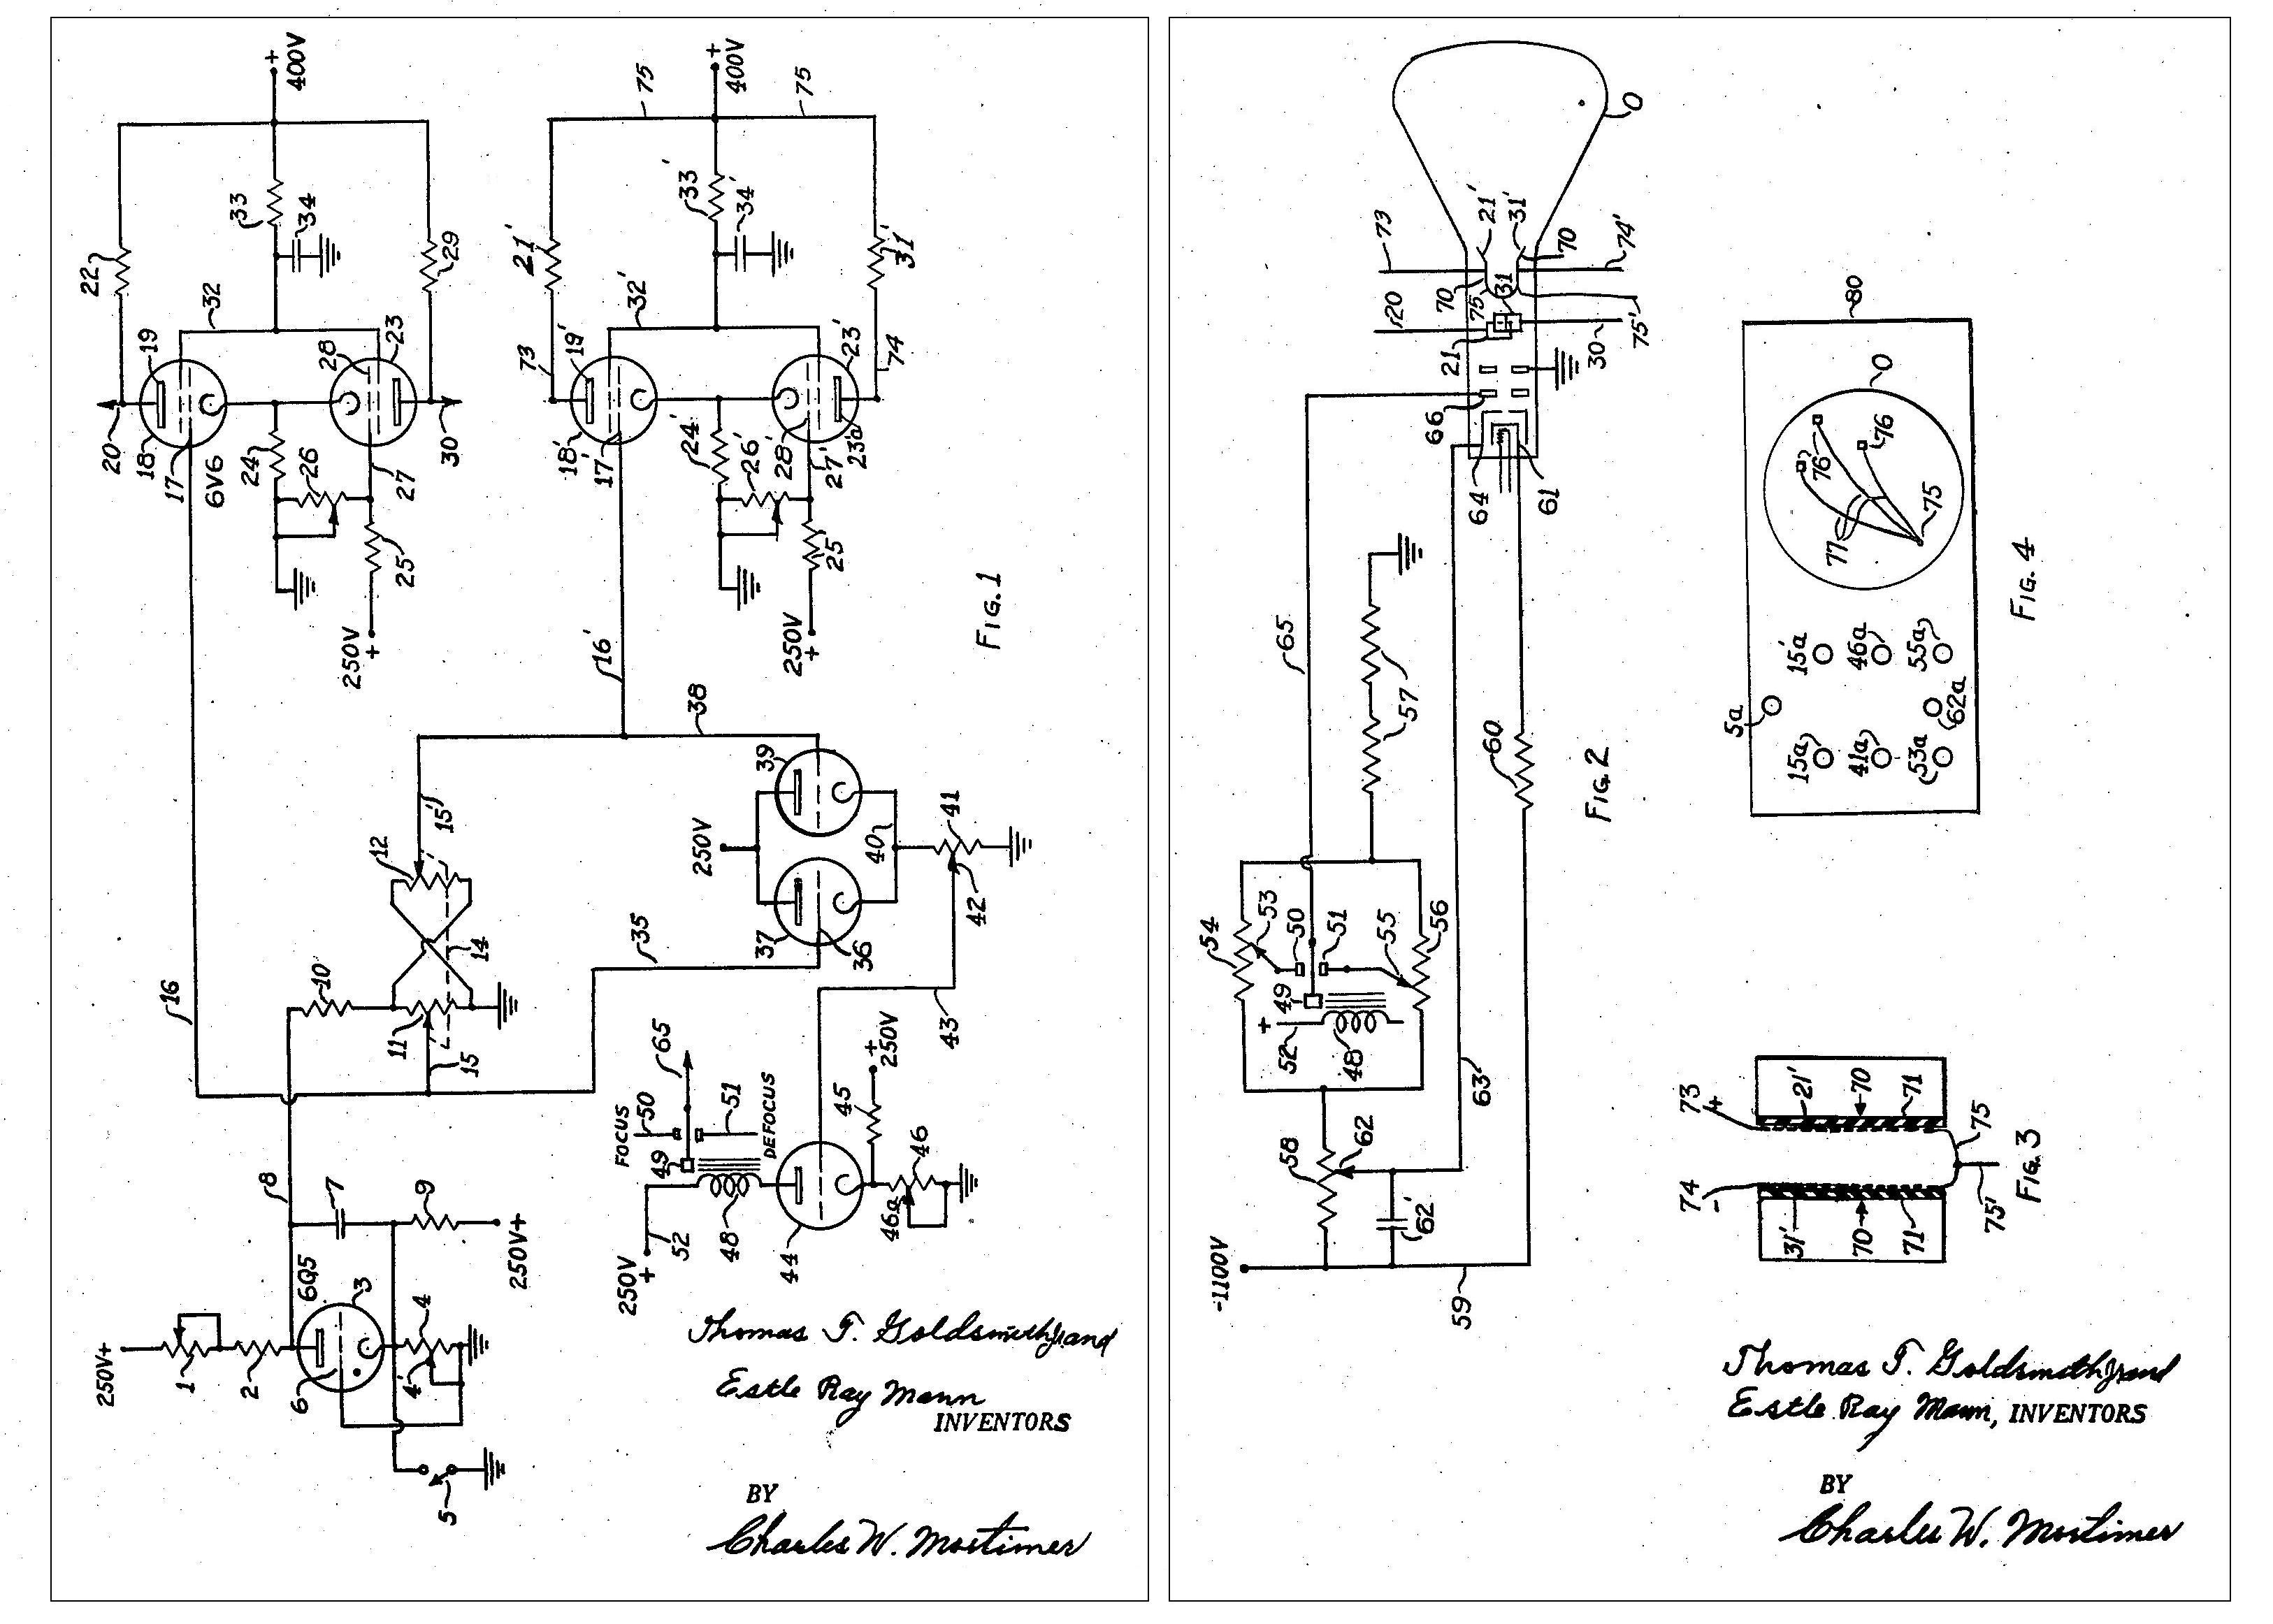
\includegraphics[width=.7\linewidth]{./figures/Cathode_ray_tube_amusement_device_-_schematic.jpg}
}

\frame{
	\frametitle{Premier jeu vidéo de l'histoire ?}
	\begin{itemize}
		\item \textbf{1958:} Tennis for two
			\begin{itemize}
				\item Entièrement analogique, se branche sur un oscilloscope
				\item Pas commercialisé
			\end{itemize}
	\end{itemize}
	\pause
	\centering
	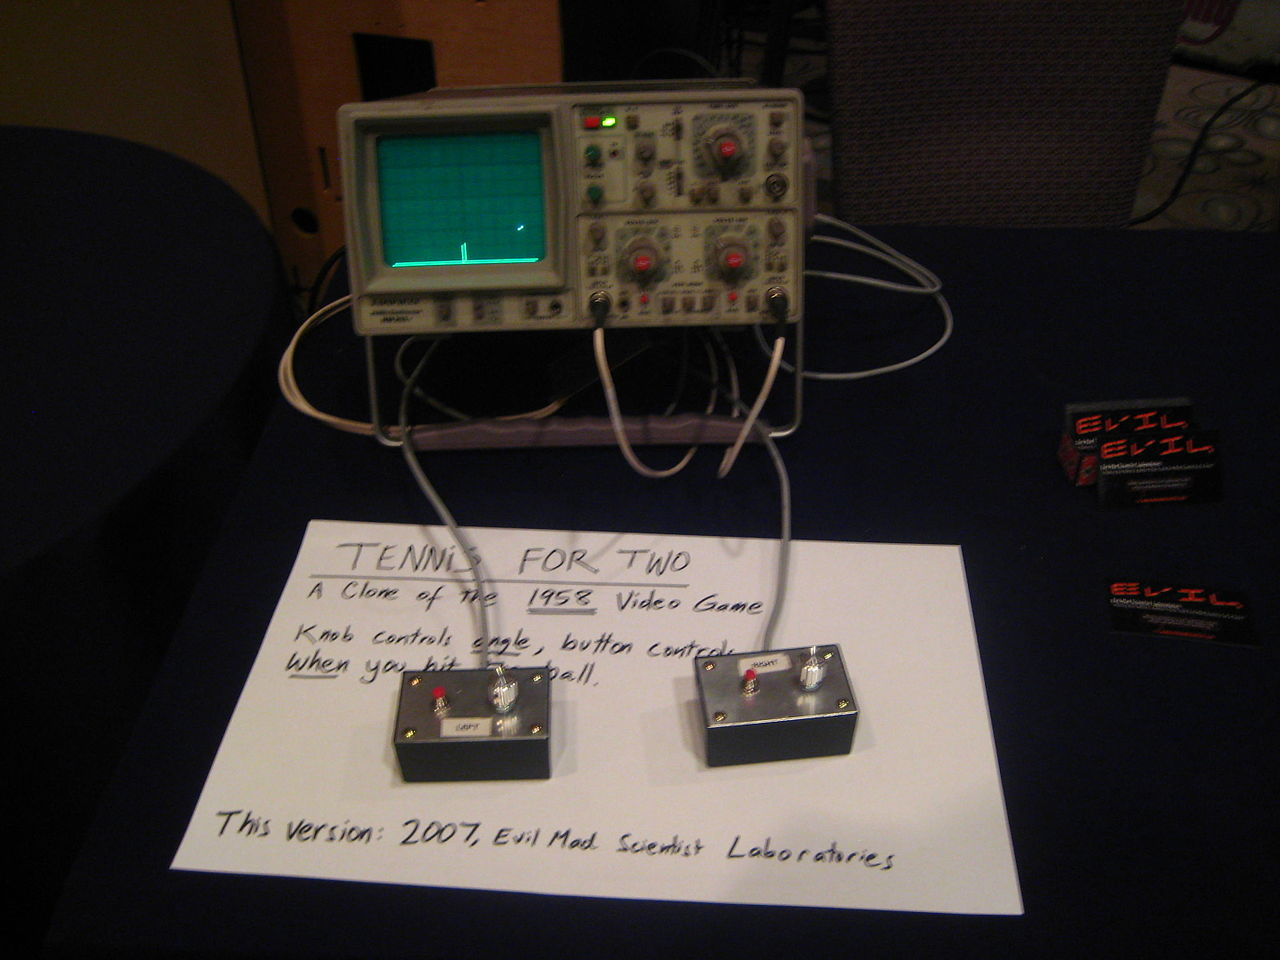
\includegraphics[width=0.8\linewidth]{./figures/Tennis_for_Two_Machine_at_CAX_2010.jpg}
}

\frame{
	\frametitle{Premier jeu vidéo de l'histoire ?}
	\begin{minipage}[b]{0.48\linewidth}
		\begin{itemize}
			\item \textbf{1972:} Pong
				\begin{itemize}
					\item Borne d'arcade, 
					\item Numérique, mais non-programmable 
					\item (micro-processeur inventé en 1971)
					\item Naissance d'Atari
				\end{itemize}
		\end{itemize}
		\vspace{2cm}
		\pause
	\end{minipage}
	\hfill
	\begin{minipage}[b]{0.48\linewidth}
		\centering
		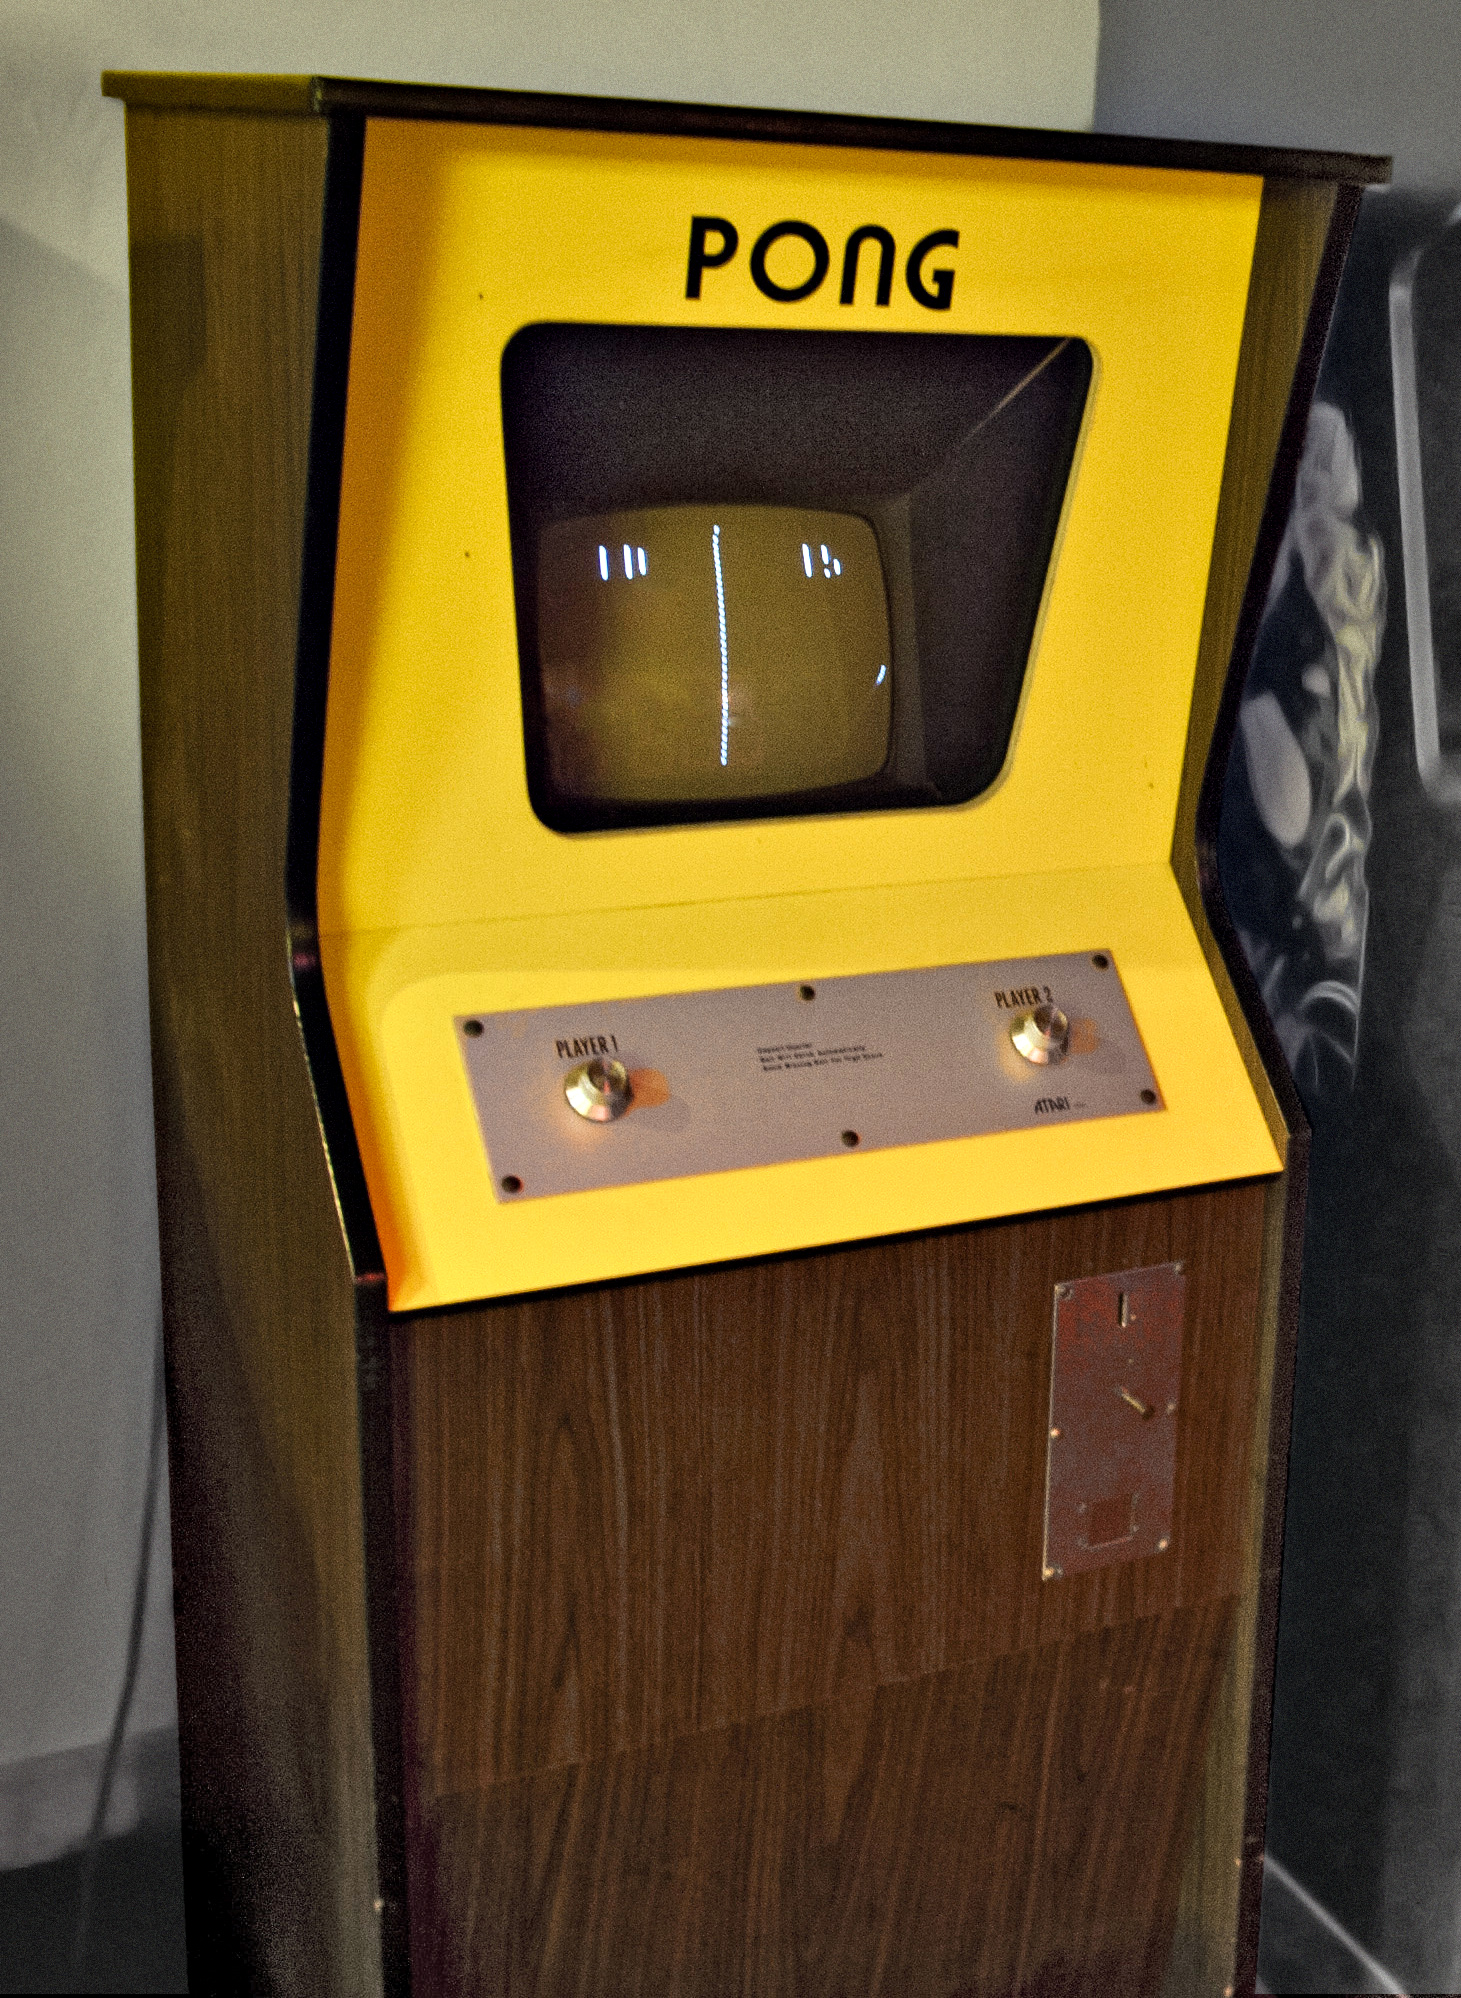
\includegraphics[width=.8\linewidth]{./figures/Atari_Pong_arcade_game_cabinet.jpg}
	\end{minipage}
}

\frame{
	\frametitle{Chronologie}
	\begin{center}
		\tiny
%		red, green, blue, cyan , magenta, yellow, black, gray, darkgray, lightgray, brown, lime, olive, orange, pink, purple, teal, violet and white.
		\begin{tikzpicture}[xscale=1.0,yscale=1.0,x=0.22cm,y=0.22cm]
			\draw[color=gray] (1970,0) grid[xstep=2,ystep=18] (2020,18);
			\draw (1970,0) grid[xstep=10,ystep=18] (2020,18);
			\foreach \x in {1970,1980,1990,...,2020} \draw(\x,0)node[below]{\x};
			\draw[fill=lightgray] (1972,16.8) rectangle (1980,15);
			\draw[align=center] (1976,15.9) node{G1 (1972,1980)};
			\draw[fill=green] (1976,14.8) rectangle (1992,13);
			\draw[align=center] (1980,13.9) node{G2 (1976,1992)};
			\draw[fill=orange] (1983,12.8) rectangle (2003,11);
			\draw[align=center] (1987,11.9) node{G3 (1983,2003)};
			\draw[fill=cyan] (1987,10.8) rectangle (2004,9);
			\draw[align=center] (1991,9.9) node{G4 (1987,2004)};
			\draw[fill=magenta] (1993,8.8) rectangle (2005,7);
			\draw[align=center] (1997,7.9) node{G5 (1993,2005)};
			\draw[fill=yellow] (1998,6.8) rectangle (2013,5);
			\draw[align=center] (2002,5.9) node{G6 (1998,2013)};
			\draw[fill=brown] (2005,4.8) rectangle (2017,3);
			\draw[align=center] (2008,3.9) node{G7 (2005,...)};
			\draw[fill=lime] (2011,2.8) rectangle (2017,1);
			\draw[align=center] (2014,1.9) node{G8 (2011,...)};
		\end{tikzpicture}
	\end{center}
}

\end{document}


